% ============================================================
%  SEZIONE 2 — Architettura
% ============================================================
\section{Architettura}

\subsection{Pattern MVC e organizzazione del progetto}
Abbiamo adottato il pattern architetturale \mvc (Model--View--Controller),
strutturato su tre livelli distinti.

\begin{itemize}
  \item \textbf{Model.} I POJO del dominio (\texttt{User}, \texttt{Training}, \texttt{Composition}, \texttt{CustomComposition}, \texttt{Review}, \ldots) e i repository gestiscono l'accesso al database H2 tramite \texttt{JdbcTemplate}. Mapper dedicati (\texttt{UserMapper}, \texttt{TrainingMapper}, \texttt{ExerciseMapper}, \ldots) si occupano della conversione da \texttt{ResultSet} a oggetto del dominio, tenendo questa logica fuori dai repository. La gestione degli utenti di sicurezza è delegata a \texttt{JdbcUserDetailsManager}, che opera sulle tabelle \texttt{USERS} e \texttt{AUTHORITIES}.

  \item \textbf{View.} I template Thymeleaf compongono le pagine HTML. I componenti comuni, intestazione, barra di navigazione, carosello delle recensioni, footer e script Bootstrap, sono estratti come fragment riutilizzabili nella directory \texttt{templates/bases/}. Il frontend usa Bootstrap~5 per il layout e Chart.js per gli istogrammi delle statistiche; le chiamate alle recensioni usano \texttt{fetch} con \texttt{async}/\texttt{await} per aggiornare la pagina senza ricaricarla. Abbiamo scelto \texttt{async}/\texttt{await} perché rispetto a \texttt{XMLHttpRequest} o alle Promise con \texttt{.then()} il codice risulta più leggibile e segue il flusso di esecuzione in modo più lineare.

  \item \textbf{Controller.} I controller gestiscono le richieste HTTP seguendo il pattern \textbf{controller $\to$ service $\to$ repository} e sono organizzati per area funzionale (\texttt{MainController}, \texttt{AdminDashboardController}, \texttt{TrainingController},\\\texttt{ReviewController}, \ldots). I service incapsulano la logica applicativa: \texttt{CheckUserService} verifica l'unicità dello username, \texttt{PlanService} valida i piani con una whitelist dei ruoli consentiti per impedire la \textit{privilege escalation} ad amministratore, \texttt{PasswordValidationService} valida il formato della password lato server, necessario perché le validazioni JavaScript lato client possono essere aggirate modificando le richieste HTTP.
\end{itemize}

\subsection{Comunicazione tra i servizi}
La web app principale comunica con il REST service tramite OpenFeign: il client \texttt{TrainingsProxy} dichiara gli endpoint del REST service come metodi Java annotati, e il framework genera l'implementazione HTTP. Il REST service espone i programmi predefiniti, la composizione di ciascun programma e il calcolo delle calorie. %, ed è in ascolto sulla porta 8081.

\subsection{Diagramma dell'architettura}
% La Figura~\ref{fig:architettura} illustra la struttura del sistema.

\begin{figure}[H]
\centering
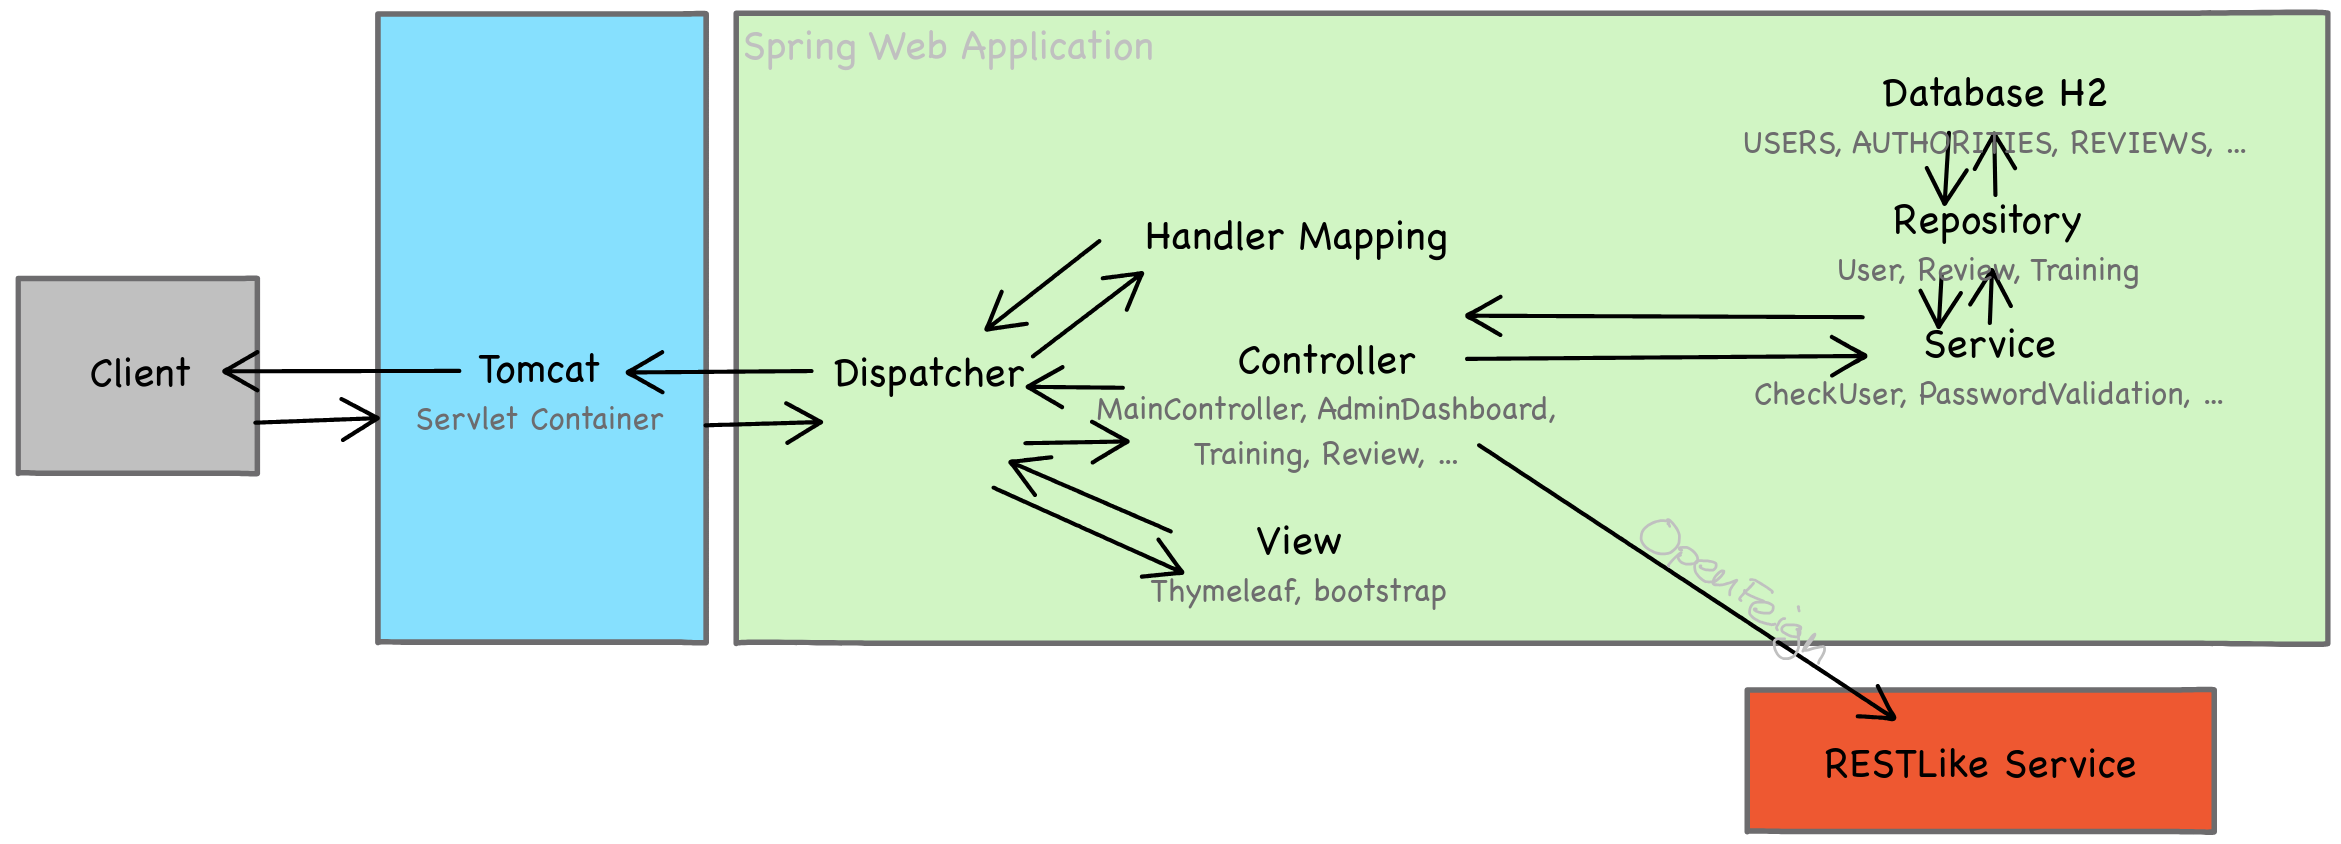
\includegraphics[width=\textwidth]{resources/architecture_schema.png}
\caption{Diagramma dell'architettura del sistema.}
\label{fig:architettura}
\end{figure}

% \begin{figure}[H]
% \centering
% \begin{tikzpicture}[
%       node distance = 0.9cm and 2cm,
%       every node/.style = {font=\small},
%       layer/.style    = {
%         draw, rounded corners=4pt, minimum width=3.2cm,
%         minimum height=1cm, align=center,
%         fill=primary!12, draw=primary!60, text=black, thick
%       },
%       arrow/.style    = {-Stealth, thick, color=primary!80},
%       dbnode/.style   = {
%         draw, cylinder, shape border rotate=90,
%         aspect=0.35, minimum width=2.2cm, minimum height=0.9cm,
%         fill=secondary!15, draw=secondary!60, align=center, font=\small
%       },
%       client/.style   = {
%         draw, rounded corners=4pt, minimum width=3.2cm,
%         minimum height=1cm, align=center,
%         fill=BrickRed!10, draw=BrickRed!50, thick
%       },
%     ]
% \node[client]  (browser) {Browser\\\textit{(Client)}};
% \node[layer,   right=of browser]  (ctrl)    {Controller\\(Routing \& Logic)};
% \node[layer,   above=of ctrl]     (view)    {View\\(Template / HTML)};
% \node[layer,   below=of ctrl]     (model)   {Model\\(Business Logic)};
% \node[dbnode,  right=of model]    (db)      {Database};
% \draw[arrow] (browser.east)  -- node[above, font=\tiny]{HTTP Request}  (ctrl.west);
% \draw[arrow] (ctrl.west)     -- node[below, font=\tiny]{HTTP Response} (browser.east);
% \draw[arrow] (ctrl.north)  -- node[right, font=\tiny]{render}  (view.south);
% \draw[arrow] (view.south)  -- node[left,  font=\tiny]{template} (ctrl.north);
% \draw[arrow] (ctrl.south)  -- node[right, font=\tiny]{call}   (model.north);
% \draw[arrow] (model.north) -- node[left,  font=\tiny]{data}   (ctrl.south);
% \draw[arrow] (model.east) -- node[above, font=\tiny]{query}  (db.west);
% \draw[arrow] (db.west)    -- node[below, font=\tiny]{result} (model.east);
% \begin{pgfonlayer}{background}
% \node[
%         draw=primary!40, dashed, rounded corners=6pt,
%         fill=primary!4,
%         fit=(ctrl)(view)(model),
%         label={[font=\footnotesize\itshape, color=primary!70]above:Server-side},
%       ] {};
% \end{pgfonlayer}
% \end{tikzpicture}
% % \caption{Diagramma dell'architettura \mvc del sistema.}
% \label{fig:architettura}
% \end{figure}

% \subsection{Struttura delle directory}
% \begin{lstlisting}[language=bash, caption={Struttura del progetto dopo il refactoring.}]
% main_webapp/
% |-- src/main/java/exam_project/main_webapp/
% |   |-- configurations/    SecurityConfig, ProjectConfig,
% |   |                      MainWebappApplication
% |   |-- controllers/       AdminDashboardController, MainController,
% |   |                      PasswordController, ProfileController,
% |   |                      ReviewController, StatisticsController,
% |   |                      TrainingController, UpgradeController
% |   |-- mappers/           DefaultTrainingCountersMapper, ExerciseMapper,
% |   |                      TrainingMapper, UserMapper, UserSummaryMapper
% |   |-- pojos/             Composition, CustomComposition, ExerciseDTO,
% |   |                      Review, SecurityUser, Training, User
% |   |-- proxies/           TrainingsProxy (OpenFeign)
% |   |-- repositories/      ReviewRepository, TrainingRepository,
% |   |                      UserRepository
% |   |-- services/          CheckUserService, PasswordValidationService,
% |   |                      PlanService, ReviewService, StatisticsService,
% |   |                      TrainingService, UserService
% |-- src/main/resources/
% |   |-- templates/
% |   |   |-- bases/         head.html, navbar.html, footer.html,
% |   |   |                  carosello.html, review.html, scripts.html
% |   |   |-- *.html         Pagine pubbliche e dashboard
% |   |-- static/
% |   |   |-- css/           style.css
% |   |   |-- js/            review.js, customTraining.js,
% |   |                      changePassword.js, signup.js,
% |   |                      loginValidation.js, carosello.js
% |   |-- application.properties
% |   |-- schema.sql
% |   |-- data.sql

% RestLike/
% |-- src/main/java/org/example/restlike/
% |   |-- Controllers/       MainController
% |   |-- Mappers/           CompositionRowMapper, ExerciseRowMapper,
% |   |                      TrainingRowMapper
% |   |-- Pojos/             Composition, Exercise, Training
% |   |-- Repository/        TrainingRepository
% |-- src/main/resources/
%     |-- schema.sql
%     |-- data.sql
% \end{lstlisting}
